\chapter{Experiments}
\label{chap:Experiments}
%\color{ForestGreen}
%\begin{itemize}
%	\item kurze einführung in die test fälle mit einer erklärung, was f1 scores sind
%	\item Alles NLP Aufgaben bei denen Bert "überraschend" gut abschneided
%	\item Jetzt mit der erweiterung zu scibert erneut betrachtet
%	\item Einföuss des vocabulars und des corpus genau gegenübergestellt
%	\item all got dropout of 0.1
%	\item loss cross entropy
%	\item optemizer adam
%	\item finetuning for 2 to 5 epochs 
%\end{itemize}
%\color{black}
In this section we will look at replication in more detail and discuss the approach and possible deviations from the original paper. So first comes the basic structure, followed by going through some examples that show us what the functions do and if our implementations work as expected. After that we will briefly talk about the hardware that was used. This is followed by a more detailed discussion of our implementation. Then we will look at some of the more serious problems and finally we will look at the obtained results.

Since the basic architecture for the underlying BERT model remains the same and does not change, we will only look at the task specific part. Furthermore, we restrict ourselves to the classification tasks and, to be more precise, to the REL task. The implementation consists of four main parts. They are the data acquisition and preprocessing, the transformer itself and last but not least the evaluation of the model with the help of a score. Here we use the F1 score to follow the original paper in this area as well. 

\subsection{Simple tests and examples}
To ensure that these individual areas function correctly and that errors have not already sneaked in. There are several outputs that show the functionality in a small scale and can ideally catch some errors. These outputs can be found in the Jupyter Notebook under Tests. In this section, the first record and the corresponding label of the training dataset are displayed first. The same is repeated for the test data set. After these examples, a dry run of the tokenizer follows. This is to assure us that the tokenize function, which puts the data into a form that the transformer can read, is working correctly. This is shown with a sentence that leads to the same result both by hand and by the function.  Next, the tokenization of special tokens is examined. This is to guarantee that the special tokens needed for the NER task are correctly recognized and translated. This is followed by some examples that test the functionality of the loss function and the embedding of the previously translated sentence. At this point, however, the verification of correctness becomes difficult, since the interpretation of the representation of the CLS token is no longer directly evaluable for humans. Although it can be shown that this process functions and presumably also operates correctly, this example no longer guarantees this.  This is followed by the tests that refer to the evaluation, in other words to the F1 score. Here we first consider whether the formats have been converted correctly so that the Metric package which is used for the calculation can read them and then we briefly compare whether the example delivers the expected F1 score. 

\subsection{Hardware requirements}
In this section, we will take a brief look at the usability of different hardware platforms for creating transformer models and training or testing them. More specifically, we will compare the google-colab environment with an Nvidia GPU and an AMD GPU. Due to the randomness of the hardware assignment on the google-colab page, the used GPU can not be defined more precisely. The utilized Nvidia GPU was a GeForce 940MX with about 2 GB of VRAM, and the AMD GPU on the other side was an RX580 with about 8 GB of VRAM. 

At this point the extent to which AMD's ROCM stack \cite{Devices2021} is usable will be briefly described, because surprisingly we were able to define the model and make predictions with it in a newly created state. Unfortunately, due to instabilities in the ROCM stack after an update that must have broken some internal dependencies that the kernel and ROCM driver must have relied on, the Linux kernel could no longer use the GPU, and so the video output of the computer was unusable.

Even though this shows that an AMD GPU is actually capable of running the Transformers.jl \cite{Cheng2020} package and loading at least a newly defined model. Even though I cannot reveal whether the model could be trained or otherwise used further. This fact in itself is surprising, since AMD itself describes the support status of the RX580 as only potentially possible \cite{Devices2021}, and Julia describes AMD GPU support as experimental. \cite{Besard2021}

However, everyone should be mindful not to use the ROCM-Stack on a productive system due to its instability, but rather only in a virtualized environment or on systems where the unusability of graphics cards will not impede the use of the system.   

This brings us to the GeForce 940MX. This graphics card unfortunately reaches its limits due to its memory size. 2GB of VRAM, of which even a little bit less is usable, does not suffice for the used BERT model nor for SciBERT and thus results in an out of memory error. Therefore, this hardware will not be considered further. 

Thus only the google-colab environment remains. 
This platform provides about 10 to 15 GB of VRAM. After the model has been moved to the graphics card, Julia shows an occupancy of just over 2 GB memory with the help of the memory indication of the CUDA driver. Here we can see why the 940MX was not able to load the model. The calculation of an epoch usually takes between 500 and 1000 seconds. These fluctuations could have several causes, but are most likely due to the google-colab environment and in particular the fact that several instances share the same graphics card. This is most likely the reason for the observed strong fluctuations from epoch to epoch. This assumption is particularly reasonable, since sometimes almost every epoch lasted the same time, apart from relatively small fluctuations of less than 50 seconds. Interestingly, the entire video memory is used for caching, even though the model consumes just over 2 GB of memory and the entire original chemprot dataset is about 5MB in size when unpacked. Still, the runtime required in the google-cab environment is about as expected and significantly faster than training on a CPU. The CPU, which was a Xeon E3-1230 v3 with four cores, needed about as long for a single step as the graphics card in the google-colab eviremont needed for an epoch. A step here consisted of only one sentence and the corresponding label.
 
\subsection{Data preprocessing}
Due to the availability of the datasets used by the original authors, we will use their prepared datasets, which are already prepared in such a way that they can be more easily used for training and still differ only slightly from the original datasets. The datasets we will use will be retrieved directly from the SciBERT GitHub page and will be made available through the DataDeps package \cite{White2019}, which provides an easy way to retrieve data that may or may not be available locally. If not already stored locally, it is cached in the local Julia path and within Julia, the DataDeps package provides the appropriate paths to the data and retrieves it from the defined source as needed. In addition, a hash can also be defined to ensure that the provided data is identical to the expected data.\cite{White2019} 

In the following section, we will take a closer look at the original data and the individual changes that were made to use these data sets for the training process. 

\subsubsection{Chemprot} 

The Chemprot data is provided in a JSON line file format. More precisely, each line consists of a text and the corresponding label. A field for metadata is also provided, but is usually not used. In its original format, the chemprot corpus consists of a develop, test, and train set, where the develop, test, and train folders correspond to the files of the same name within the chemprot folder provided on SciBERT's GitHub page. The difference arises from the database-like structure in which the chemprot corpus is originally provided, those subdivided sets of information are, for example, the text itself that is in one file and the positions and annotations are in another. These subdivided information sets have been merged by \citeauthor{Beltagy2019} and are provided in a single file in the format mentioned earlier. \cite{Beltagy2019,Wang2016} 

Since the data is already very close to the format that is needed for the transformer, only small changes have to be made. These consist mainly of not changing the special tokens that are already included in the data by the tokenizer or wordpiece. Afterwards these preprocessed sentences should only be changed by using the vocabulary function. This takes place in the tokenize function, which first locates the special tokens and finds out which pair comes first. This is followed by splitting the sentence at the locations of the special tokens. Now these subsets are processed by the tokenizer and by wordpiece and then reassembled together with the corresponding special tokens to form a whole sentence. After that the numeric representation is generated by the vocabulary and the segment representation is generated together with the corresponding mask. The segments always get ones, because we only process single sentences with this function and the mask is created with the mask function from the Transformers.jl \cite{Cheng2020} package. Now only the correct labels are missing. These are put into a 1 out of k scheme using the onehot function from Flux. \cite{Flux.jl-2018,innes:2018} For this function we need the correct label and an array with all existing labels. This array has already been defined based on all the labels found in the training data. With all this data we now have all the prerequisites to continue with the transformer. 

%\section{Classification tasks}
%Both classification tasks use the same architectural structure. This means that the final BERT or SciBERT layer is followed by a dense or fully connected linear layer. This dense layer then acts as the linear classification layer described in the original work. 
%\subsection{Text Classification (CLS)}
%Classic sequence classification tasks or text classification tasks, as they are called in the original paper, can be implemented in Julia without any particular challenges. Especially since the data is already available in a format that mostly only needs to be loaded and the task is only a transformation from a text to a single label. Together with the architecture for classification tasks already described, this makes the implementation of this task very easy. We just need to combine Bert and the classification layer and provide this model with the text and the label in the correct formats. This means, on the one hand, adding the "[CLS]" and "[SEP]" tokens to the text after preparing the text with the tokenizer and wordpiece and, on the other hand, preparing the labels in a format that can be read by the model, which transforms them into a "OneHotMatrix" for "Flux", corresponding to a one out of k representation per sequence.
%\subsection{Relation Classification (REL)}

\subsection{Implementation of the replication}
The first step, which belongs to the actual replication, is to rebuild the original transformer. For this we first need the basic model. We use Transformers.jl\cite{Cheng2020} for this task and some others that are still to come. This package includes some very helpful functions for handling transformers. These range from loss functions to wrappers that make it much easier to create new transformers. We therefore use Transformers.jl to load the base model and use set Classifier to replace the layers previously required for NSP and MLM with the ones we need. For the REL task, this means that the actual BERT architecture, as shown in the figure \ref{fig:bert}, should get an additional classifiaction layer. Here we use a dropout of 0.1 as described in the original paper. At this point we deviate somewhat from the original paper, which describes that the CLS layer is passed directly to the classifier layer.\cite{Beltagy2019} We realize this by using the loss function, which only passes forward the representation of the CLS token to the classification layer and not the representations of all individual tokens. We will discuss the loss function in more detail in the following. Another remark would be that here the classification layer is realized by a Dense layer using the Flux library. This layer can be seen as a fully connected one.  Now the optimizer is missing, which the same as in the orginal one namely Adam. The batch size will be set to 1 due to the implementation here. This differs from the original paper which used 32.\cite{Beltagy2019} The main reason for this decision was that it created some problems using mini batches and so far not all of them could be solved. For this reason all following results will use a batch size of 1. 

With this we move on to the loss function. This not only takes over the task of an actual loss function, in other words to calculate an error between the prediction of the model and the real label, but also deals with how the data flows through the model. This can be seen by the fact that both the embed and transform steps are done explicitly here. This allows us to simply call our loss function with the corresponding label and dataset and get the corresponding value for the loss. For the actual loss calculation, we use the logitcrossentropy as opposed to the crossentropy that was used in the original paper.\cite{Beltagy2019} This decision was made because the crossentropy functions here expect values between 1 and 0 that sum up to 1, and this would be achieved, for example, by using a softmax layer. However, performing these two steps by hand is numerically more unstable than using the logitcrossentropy function that incorporates these two functions. \cite{Flux.jl-2018,innes:2018}

Apart from the loss, we need one more function, which is the function that computes a score for the task. In the case of the REL tasks this will be the F1 micro score. We calculate this score using the Metrics.jl \cite{Kumar2020} library. For this we need to collect all the predictions for the test data, the predictions themselves are analogous to the process described for the loss function. Furthermore we need the real label and this combination of label and prediction must now be converted into a certain format, from this the F1 micro score can be calculated directly using the 'f\_beta\_score' function from the Metrics package. \cite{Kumar2020}
Now only the actual training is missing. For this two loops are used, one corresponding to the epochs and the other to the index in the training dataset. At this point different statistics are calculated and saved for later analysis. These include memory usage, runtime and F1 score per epoch as well as loss for each training step. 

This training process is then performed for several models and for different learning rates. This leads us then to our results. 

\subsection{Complications}
In the following, we briefly review some of the problems we have encountered during this work. The order follows that of the information flow in the model, starting with the input data and ending with the output. 

After this sequence the first problem is to transform the data, which contains already the two text sections that are marked with the special tokens "[\textless\textless]", "[\textgreater\textgreater]", "[~[[~]" and "[~]]~", these sentences must be processed by the tokenizer and by wordpiece, but without changing the mentioned tokens. If the individual sentences were processed without further precautions, the special tokens would be modified as well. However, due to this alteration, these tokens would no longer be interpreted as special tokens by the vocabulary, but would be seen as "normal" words. To avoid this, the tokenize function was written that splits the text into partitions and processes them individually using the tokenizer and wordpiece. This was necessary primarily because partitions identified by a pair of corresponding special tokens might not have the same length after processing. Due to this potential variation in segment length, it is not directly possible to find the new position of the tokens based on the old one and simply add them manually. Instead, the individual sections separated by the special tokens are processed one by one and then the special tokens are placed in between the corresponding segments. This procedure is based on the addition of the "[CLS]" and "[SEP]" tokens in the CLS, but extends it. 

The next problem follows directly the one described before. The individual records of the data sets sometimes consist of characters that do not occupy only one code unit and so problems can occur when the end of a string is expected to be at the position of the length of the string. A code unit here describes a fixed size in memory that is generally required for encoding a single character. Fortunately, an error is generated when attempting to create a view of a string that ends or begins in the middle of a character that spans multiple code units. Although the error is relatively vague, a closer look at the string quickly reveals that the error occurs near special characters. With this knowledge, because of the different number of code units sometimes required to encode special characters, one can quickly find the explanation and underlying problem in the appropriate documentation. Here the functions 'firstindex' and 'lastindex' or the function 'split' can help. All these functions take into account the differences between position and code unit. 

Another, more general problem was that some packages provide very few examples of how they should be used, and at the same time are not sufficiently detailed in the specifications. This leaves unanswered questions that initially prevent the packages from being used. For example, the MLBase package provides many different metrics, but requires an object of type ROCNums for computation. This type can be generated by the MLBase package, but the documentation only says that a ground truth and the predictions of the model are needed as input. However, the documentation for the actual ROCNum type says nothing about the format in which these two pieces of information must be provided, and there is nothing at all about the ROCNum type in the examples. With a little luck, however, one comes across the documentation of the Confusion matrix, which contains an example of how to create a ROCNum object. Using this example, one can then derive the correct formats. However, missing information of this type can be found multiple times in diffrent packages and requires either some luck to find a working example, or trial and error to eventually hopefully figure out the correct format.  Another example of such a problem, was the gradient calculation. In the official documentation of the Transformers.jl package there are still outdated examples that no longer work, and so you are quickly faced with the problem of not knowing why a certain part doesn't work. To be exact, it was relatively easy to find out which part of the code is not working as it should, but a very big problem was the assumption that the not working part should work, because it was only a function call and it corresponded one to one to the official documentation. Only later by a forum contribution of the developer himself it became clear that this function does not supply the necessary information any more and thus in our case the update step did nothing. A warning would have been appropriate here that the function call does not work anymore. In this case, a note that some information in the documentations are still missing or a hint that the documentation or the examples do not work anymore because they are outdated would have been very helpful. Especially since one example seems to work, it would have been important for it to stand out in some way from the ones that are no longer working, and to not give the impression that they all are still up to date.

\begin{figure}[h]
	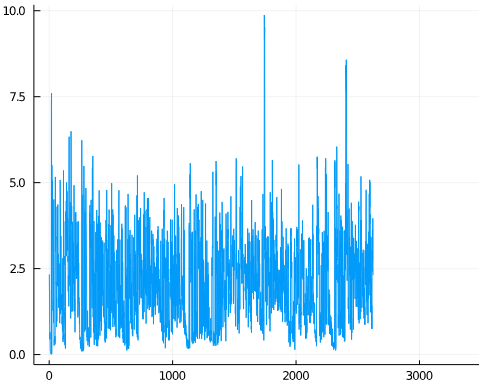
\includegraphics[width=\linewidth]{src/losses}
	\caption{The calculated loss for the REL experiment using SciBERT with the scivocab vocabulary. Each x-axis step represents one training step. 
		It can be seen that the loss does not decrease and is no longer displayed from a little more than 2500 steps. This is due to the fact that the calculated loss results in NaNs from this point on.}
	\label{figure:loss}
\end{figure}

\subsection{Observed results}
Now we briefly come to the results we observed. Here it is noticeable that after a few thousand steps only NaNs are obtained as loss. As soon as NaNs appear, they should result in the fact that no further training is possible, since the training is based on the difference between the calculated result and the expected result. If this difference cannot be determined, no further update step will be possible. The NaNs can also be seen in figure \ref{figure:loss} .There they are represented by the suddenly stopping curve, which should show a few thousand additional steps, but the plot function does not visualize NaNs.
The NaNs that are generated here seem to be created internally within the CUDA environment. Especially since all inputs were considered exemplary for the model and they seem to be correct so far, it is reasonable to assume that there might be an incompatibility between the software components causing the NaNs here. Since some parts of the software packages used here are still under very active development, this might have resulted in bugs sneaking in. On the other hand it could be a problem caused by outdated software, for example since we have no direct control over the software used in the Google-Colab environment this is another possible source of errors. Another possibility would be numerical instabilities resulting in NaNs. However, this seems relatively unlikely since explicit approaches were used here to fix exactly these numerical weaknesses. Last but not least, there could also be an error in the implementation. This possibility is opposed by the individual intermediate steps, which exemplify the correct functionality. In particular the fact that the input, which the model receives, can be directly observed and no obvious errors are found there.

Another important observation here is that the NaNs are already present in the model, i.e. do not arise from the loss function, but are already present in the last layer of our model and are only transported further from here. This again speaks for the first or last assumption.


